\documentclass{jib}
\newlength{\platz}
\setlength{\platz}{15pt}
\RequirePackage{listings}
\lstset{%
  basicstyle=\ttfamily,
  fontadjust,
  flexiblecolumns=true,
  frame=L,
  xleftmargin=15pt,
  framesep=5pt,
  emphstyle=\rmfamily\itshape}

\usepackage{pdfpages}

%%%%%%%%%%%%%%%%%%%%%%%%%%%%%%%%%%%%%%%%%%%%%%%%%%%%%%%%%%
% JIB Header/Footer
%%%%%%%%%%%%%%%%%%%%%%%%%%%%%%%%%%%%%%%%%%%%%%%%%%%%%%%%%%
\jibvolume{XX} % insert volume
\jibissue{X}   % insert issue
\jibpages{XXX} % insert article ID
\jibyear{XXXX} % insert year
\makeHeaderFooter{} % leave as is
%%%%%%%%%%%%%%%%%%%%%%%%%%%%%%%%%%%%%%%%%%%%%%%%%%%%%%%%%%

\begin{document}

%%%%%%%%%%%%%%%%%%%%%%%%%%%%%%%%%%%%%%%%%%%%%%%%%%%%%%%%%%
%
% Title Page
%
%%%%%%%%%%%%%%%%%%%%%%%%%%%%%%%%%%%%%%%%%%%%%%%%%%%%%%%%%%

\begin{jibtitlepage}

\jibtitle{The Simulation Experiment Description Markup Language (SED-ML):\\
Language Specification for Level~1 Version~5}


% Please make sure to use unique footnote characters for each author
\jibauthor{%
  Lucian P. Smith\iref{uw},
  Frank T. Bergmann\iref{heidelberg},
  Alan Garny\iref{auckland},
  Tom\'{a}\v{s} Helikar\iref{nebraska},
  Jonathan Karr\iref{sinai}
  David Nickerson\iref{auckland},
  Herbert Sauro\iref{uw},
  Dagmar Waltemath\iref{greifswald}, and
  Matthias K{\"o}nig\iref{humboldt},
}

%\addjibinstitution{imbio}{IMBio, Ralf Hofest\"adt, Bielefeld University, Faculty of Technology, Bioinformatics Department, D-33501 Bielefeld, Germany, \url{http://www.imbio.de}}
\addjibinstitution{uw}{University of Washington, USA}
\addjibinstitution{heidelberg}{BioQUANT/COS, Heidelberg University, Germany}
\addjibinstitution{auckland}{Auckland Bioengineering Institute, The University of Auckland, New Zealand}
\addjibinstitution{nebraska}{University of Nebraska, USA}
\addjibinstitution{sinai}{Icahn School of Medicine at Mount Sinai, USA}
\addjibinstitution{greifswald}{University of Greifswald, Germany}
\addjibinstitution{humboldt}{Humboldt University, Germany}

\end{jibtitlepage}


% adjusts the width of the abstract, please do not change!
%\begin{adjustwidth}{}{1cm} %LS NOTE:  'adjustwidth' not recognized in my setup.

\renewcommand{\baselinestretch}{1.0}
\abstract{
Modern biological research is increasingly informed by computational simulation experiments, which necessitate the development of methods for annotating, archiving, sharing, and reproducing the conducted experiments.  These simulations increasingly require extensive collaboration among modelers, experimentalists, and engineers. The Minimum Information About a Simulation Experiment (MIASE) guidelines outline the information needed to share simulation experiments. SED-ML is a computer-readable format for the information outlined by MIASE, created as a community project and supported by many investigators and software tools.

Level~1 Version~5 of SED-ML expands the ability of modelers to define simulations in SED-ML using the Kinetic Simulation Algorithm Onotoloy (KiSAO).  While it was possible in Version~4 to define a simulation entirely using KiSAO, Version~5 now allows users to define tasks, model changes, ranges, and outputs using the ontology as well.

SED-ML is supported by a growing ecosystem of investigators, model languages, and software tools, including various languages for constraint-based, kinetic, qualitative, rule-based, and spatial models, and many simulation tools, visual editors, model repositories, and validators.

Additional information about SED-ML is available at \url{https://sed-ml.org/}.}

%\end{adjustwidth} % please do not change %LS NOTE:  'adjustwidth' not recognized in my setup.


% Include your PDF document
\clearpage
\setlength{\voffset}{0cm}
\setlength{\hoffset}{0cm}
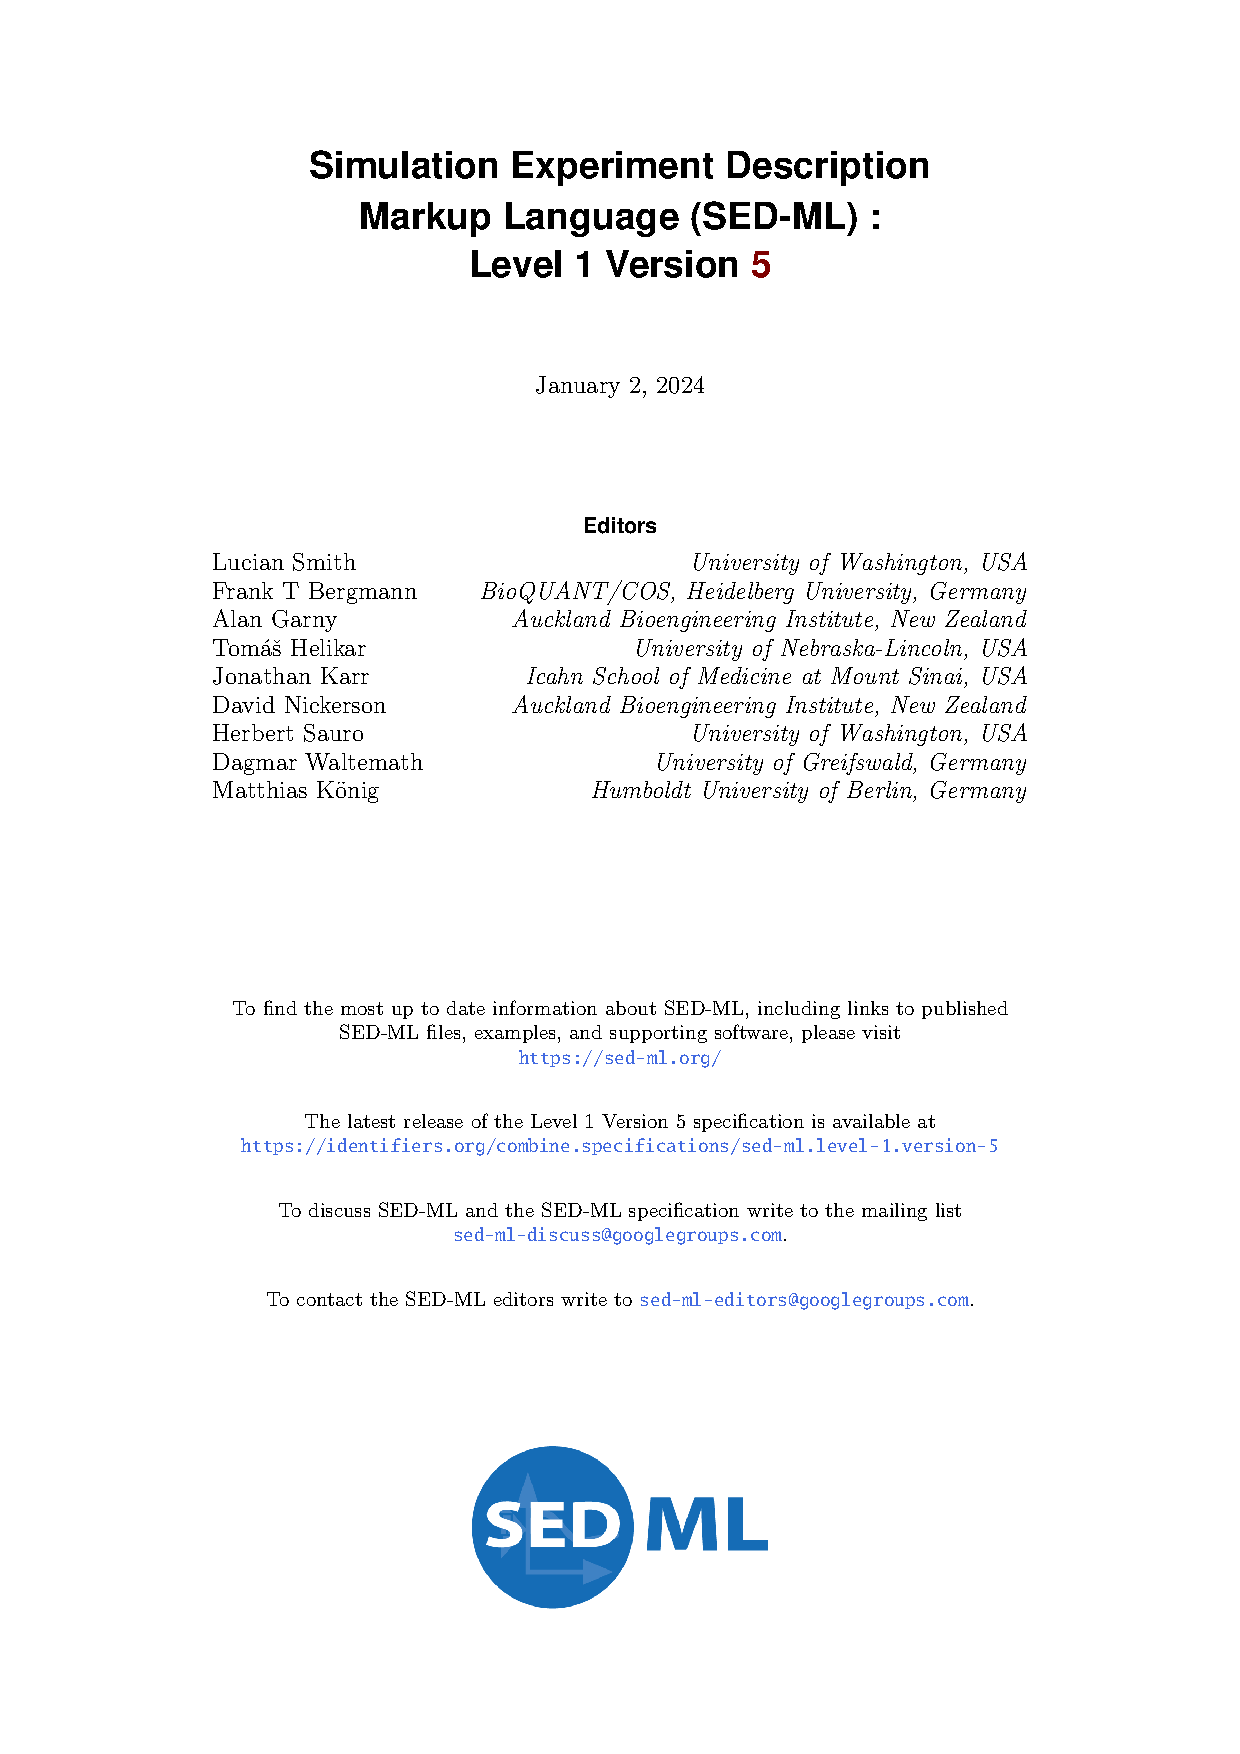
\includepdf[pages=-]{sed-ml-L1V5.pdf}

\end{document}
